%% LyX 2.0.3 created this file.  For more info, see http://www.lyx.org/.
%% Do not edit unless you really know what you are doing.
\documentclass[a4paper,english]{article}
\usepackage[T1]{fontenc}
\usepackage[latin9]{inputenc}
\usepackage{float}
\usepackage{graphicx}

\makeatletter

%%%%%%%%%%%%%%%%%%%%%%%%%%%%%% LyX specific LaTeX commands.
\pdfpageheight\paperheight
\pdfpagewidth\paperwidth

%% Because html converters don't know tabularnewline
\providecommand{\tabularnewline}{\\}

\makeatother

\usepackage{babel}
\begin{document}

\title{Fedux}

\maketitle



\part{Arranque}

Arranque Una vez cargado la imagen de disco en un emulador o iniciado
el sistema de forma nativa, aparecer� la pantalla del GRUB solicitando
la elecci�n de un kernel a bootear. En este caso la �nica opci�n es
\textquotedblleft{}Fedux Kernel\textquotedblright{} que permite continuar
el arranque del TPE.

\begin{figure}[H]
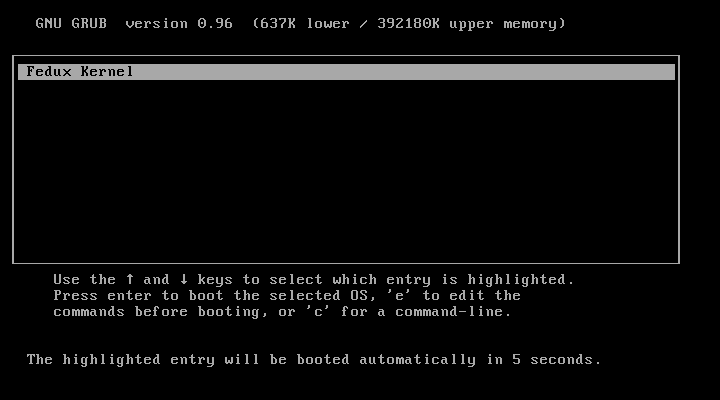
\includegraphics[scale=0.5]{bootloader}

\caption{GRand Unified Bootloader - Bootloader predilecto de los desarrolladores
de Fedux}
\end{figure}



\part{L�nea de comandos}

Una vez iniciado, el sistema presenta al usuario con un int�rprete
de comandos b�sico. Este int�rprete provee de 5 programas ejecutables
y tambi�n contiene funcionalidad para dos conjuntos de atajos del
teclado. En esta secci�n podr� encontrar la informaci�n necesaria
para interactuar con Fedux.


\section{Distribuci�n de telcado}

Puede seleccionarse la distribuci�n de teclado a utilizar ingresando
alguna de las siguientes distribuciones de teclas:

\begin{table}[H]
\begin{tabular}{|c|c|}
\hline 
Combinacion de teclas & Lenguaje\tabularnewline
\hline 
\hline 
ALT + S & Espa�ol\tabularnewline
\hline 
ALT + E & Ingl�s\tabularnewline
\hline 
\end{tabular}

\caption{Combinaciones de teclas segun la distribucion a utilizar}
\end{table}


La distribuci�n seleccionada puede visualizarse en la parte superior
de la pantalla.

\begin{figure}[H]
Poner aca la foto

\caption{Distribucion de teclas en uso}
\end{figure}



\section{M�ltiples terminales}

El sistema provee m�ltiples terminales que permiten mantener varios
historiales de trabajo. Por defecto, la terminal inicial es la n�mero
1. Puede navegar entre terminales utilizando la combinacion de teclas
ALT + {[}NUMERO DE TERMINAL{]} para seleccionar la que desee. Es importante
notar que, aunque es posible mantener m�ltiples historiales de trabajo,
no es posible ejecutar m�s de un comando en simult�neo. El �nico programa
en ejecuci�n imprime su salida en la terminal activa definida por
el usuario.


\section{Comandos disponibles}

Fedux est� provisto por defecto de algunos programas que dan algunas
funcionalidades importantes. Estos son los siguientes.


\subsection{help}

Imprime la lista de programas que se pueden ejecutar en la shell junto
con sus argumentos.


\subsubsection*{Opciones}
\begin{itemize}
\item --version (opcional) Imprime la versi�n del programa.
\end{itemize}

\subsection{echo}

Imprime los argumentos que recibe por salida est�ndar, separados por
un espacio. Para preservar los espacios, puede escribir los argumentos
entre comillas. En caso contrario, tal como lo define el est�ndar
POSIX, no se tendr�n en cuenta los espacios entre argumentos.


\subsubsection*{Opciones}
\begin{itemize}
\item -n (opcional) No imprime un caracter de nueva l�nea al final
\item --version (opcional) Imprime la versi�n del programa
\end{itemize}

\subsection{chat}

Permite la comunicaci�n entre dos computadoras a trav�s del puerto
serie.


\subsubsection*{Opciones}
\begin{itemize}
\item --version (opcional) Imprime la versi�n del programa.
\end{itemize}
\begin{figure}[H]
Poner aca una foto del chat

\caption{Fedux chat}


\end{figure}



\subsection{laws}

Programa que imprime en pantalla las 3 leyes de la rob�tica de Isaac
Asimov. Es el programa m�s basico y demustra simplemente el uso de
la funci�n printf para imprimir texto en pantalla.


\subsubsection*{Opciones}
\begin{itemize}
\item --version (opcional) Imprime la versi�n del programa.
\end{itemize}

\subsection{fortune}

Imprime una frase aleatoria tomada de una lista est�tica de frases.


\subsubsection*{Opciones}
\begin{itemize}
\item --version (opcional) Imprime la versi�n del programa.
\end{itemize}

\subsection{cowsay}

Imprime una vaca en pantalla mencionando el texto pasado por argumento.


\subsubsection*{Opciones}
\begin{itemize}
\item --version (opcional) Imprime la versi�n del programa.
\item --help (opcional) Imprime un texto de ayuda del programa.
\item -b \textquotedblleft{}Modo Borg\textquotedblright{}, usa == en lugar
de oo para los ojos de la vaca.
\item -d \textquotedblleft{}Muerta\textquotedblright{}, usa XX.
\item -g \textquotedblleft{}Codiciosa\textquotedblright{}, usa \$\$.
\item -p \textquotedblleft{}Paranoica\textquotedblright{}, usa @@.
\item -s \textquotedblleft{}Drogada\textquotedblright{}, usa {*}{*} para
representar los ojos rojos y una U como una lengua hacia afuera
\item -t \textquotedblleft{}Cansada\textquotedblright{}, usa --.
\item -w \textquotedblleft{}Enchufada\textquotedblright{}, usa OO.
\item -y \textquotedblleft{}Juvenil\textquotedblright{}, usa .. para representar
ojos m�s peque�os.
\end{itemize}
\begin{figure}[H]
Poner aca una foto de la vaca loca.

\caption{cowsay}
\end{figure}

\end{document}
